\documentclass[12pt, a4paper, oneside]{ctexart}
\usepackage{amsmath, amsthm, amssymb, bm, color, framed, graphicx, hyperref, mathrsfs, float}
\pagestyle{plain}

% multi-column
\usepackage{tasks}
% itemize
\NewTasksEnvironment[label=(\arabic*), label-width=3ex]{exercise}

\everymath{\displaystyle}

\title{\textbf{第二次随堂测试}}
\author{U08M11002 Fall 2023}
\linespread{1}
\definecolor{shadecolor}{RGB}{241, 241, 255}

\newcounter{problemname}
\newenvironment{problem}{\stepcounter{problemname}\par\noindent\textbf{题目\arabic{problemname}. }}{\\\par}
\newenvironment{warning}{\begin{shaded}\par\noindent\textbf{提交作业方式:}}{\end{shaded}\par}

\begin{document}

\maketitle

\hspace{1em}

\begin{problem}
证明  $\int_{-\infty}^{\infty} f(t) \delta(t-t_0) dt = f(t_0)$.
\quad
\end{problem}

\begin{problem}
证明:微分、积分(变上限积分)和延时器都是线性系统。\par
\begin{exercise}
	\task 微分:$y(t)=\frac{{\rm{d}}f(t)}{{\rm{d}}t}$,指函数在$t$点处(趋近于无穷小)的变化量。
	\task 积分(变上限积分):$y(t)=\int_{-\infty}^{t}f(\tau){\rm{d}}\tau$,
	      直观地理解,函数在$[-\infty,t]$区间上的面积值。
	\task 延时器:$y(t)=f(t-t_0)$,将输入信号按照$t_0$时间延迟后输出。
\end{exercise}
\quad
\end{problem}

\begin{problem}
证明以下系统不是时不变系统(LTI):
\begin{exercise}(2)
	\task (变系数)$y=tf(t)$
	\task (反转)$y=f(-t)$
	\task (伸缩)$y=f(\alpha t)$
\end{exercise}
\quad
\end{problem}

\begin{problem}
	求下图中 $f_1(t)$ 和 $f_2(t)$ 的卷积。
	\begin{figure}[H]
		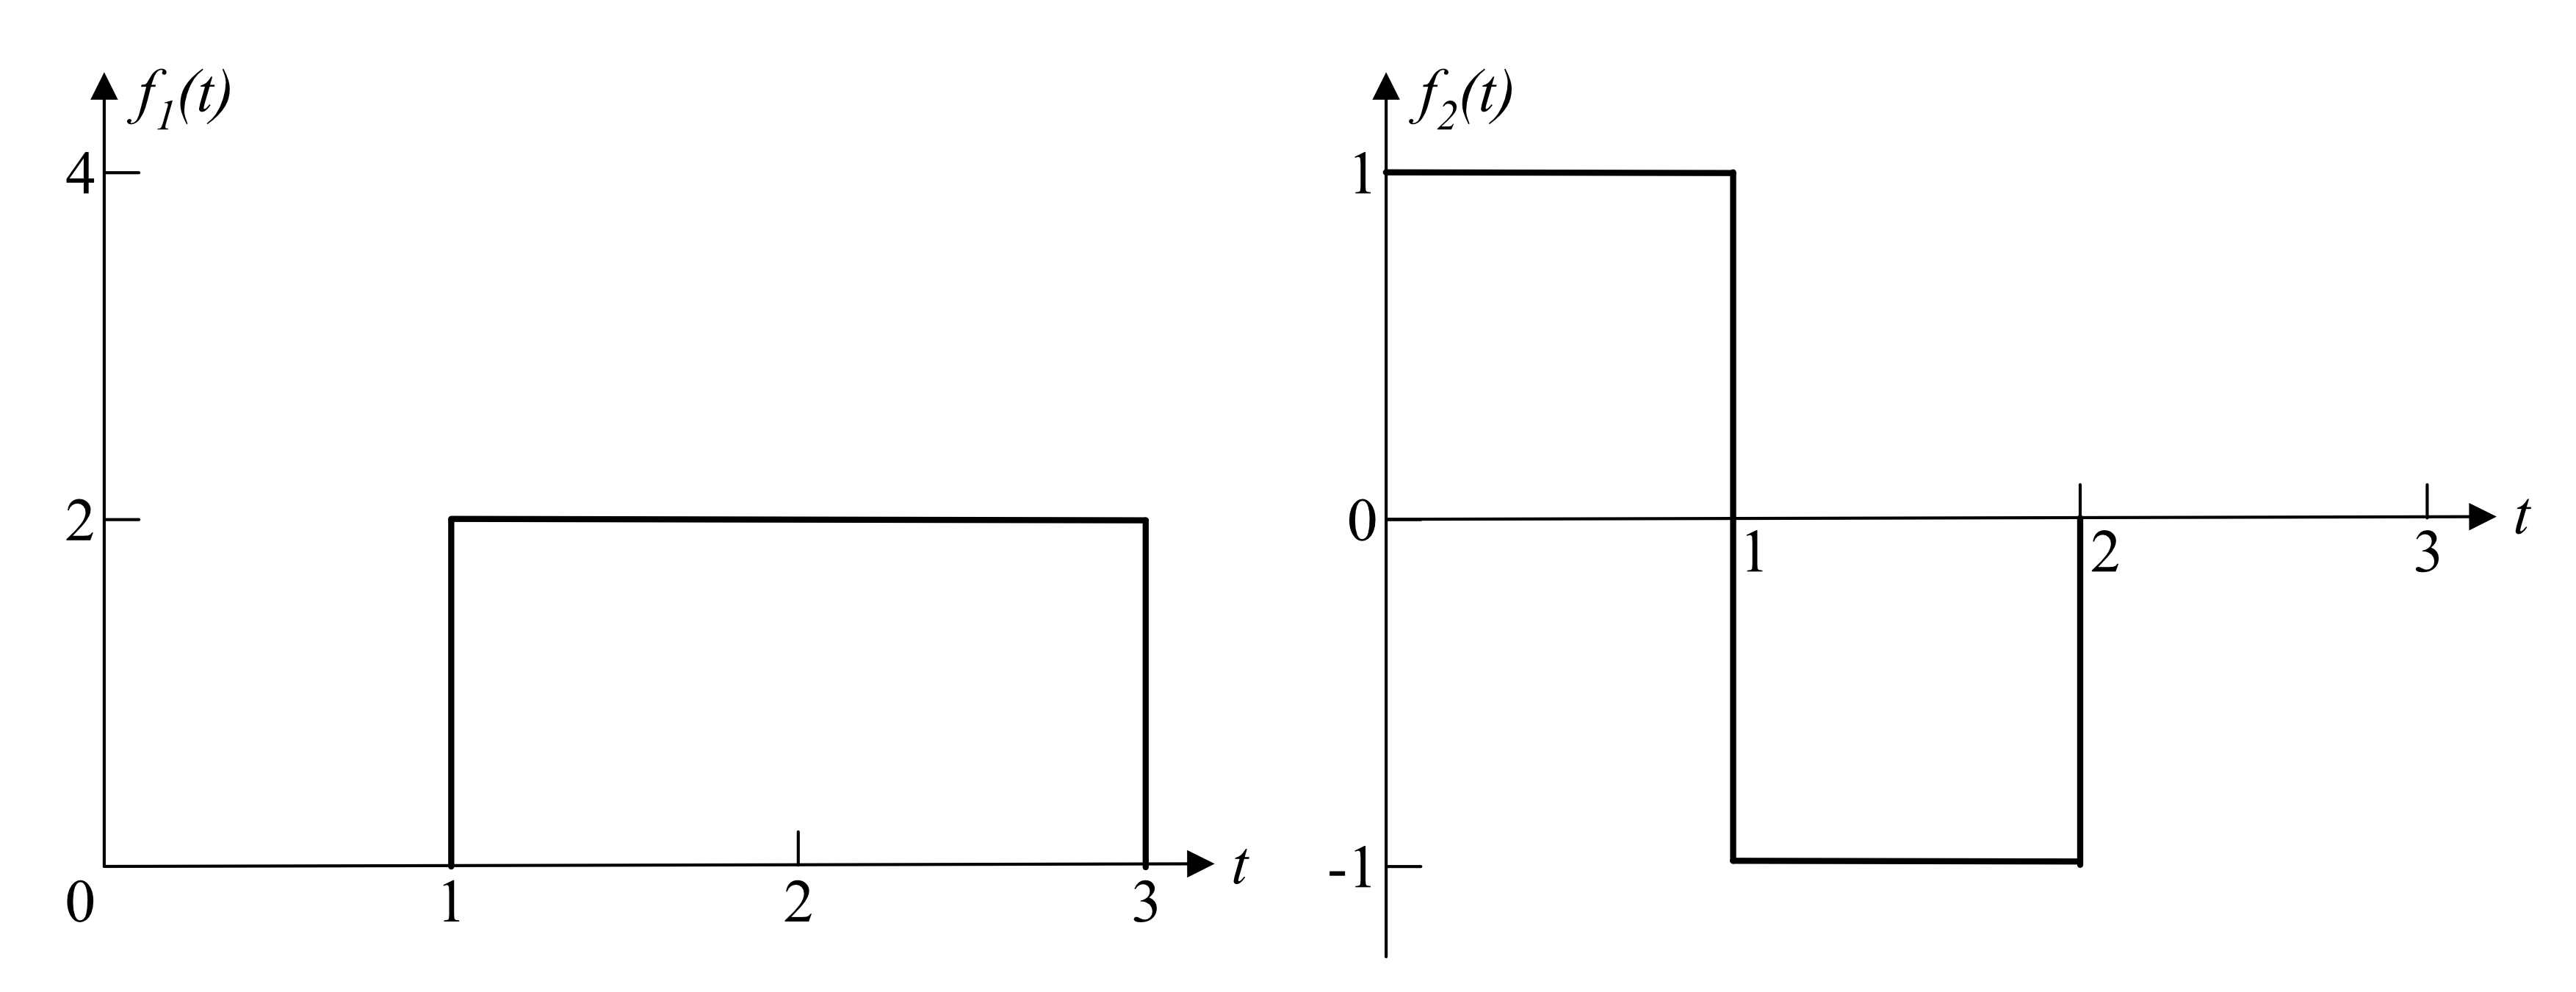
\includegraphics[width=8.5cm]{assets/hw3img1.png}
		\centering
	\end{figure}
\quad
\end{problem}

\end{document}